\documentclass{article}
\usepackage{graphicx}
\usepackage{amsmath}
\usepackage{amsfonts}
\usepackage{geometry}
\usepackage{float}

\geometry{a4paper, margin=1in}

\title{Relatório sobre Análise de Componentes Principais do Conjunto de Dados Olivetti Faces}
\author{Eduardo Henrique Basilio de Carvalho}
\date{\today}

\begin{document}

\maketitle

\section{Introdução}
Este relatório resume a aplicação da Análise de Componentes Principais (PCA) no conjunto de dados Olivetti Faces.
O objetivo foi realizar a redução de dimensionalidade e avaliar seu impacto em uma tarefa de classificação subsequente. 

\section{Carregamento de Dados e Exploração Inicial}
O conjunto de dados Olivetti Faces foi carregado, consistindo em imagens e rótulos correspondentes.
A forma original da matriz de características $X$ era $(400, 4096)$. 
Estes correspondem a 400 imagens, cada uma representada por um vetor achatado de 4096 valores de pixel (imagens 64x64). 

\section{Aplicação do PCA e Redução de Dimensionalidade}
O PCA foi inicialmente aplicado para reduzir a dimensionalidade do conjunto de dados para 100 componentes.
\begin{itemize}
    \item Os dados originais $X$ possuíam 4096 dimensões. 
    \item Após aplicar o PCA com $n_{componentes} = 100$, os dados transformados $X_{pca}$ possuíam a forma $(400, 100)$. 
\end{itemize}
Os autovalores, representando a variância explicada por cada componente principal, foram extraídos.
Um gráfico de scree (scree plot) foi gerado plotando esses autovalores em ordem decrescente. 

\begin{figure}[H]
    \centering
    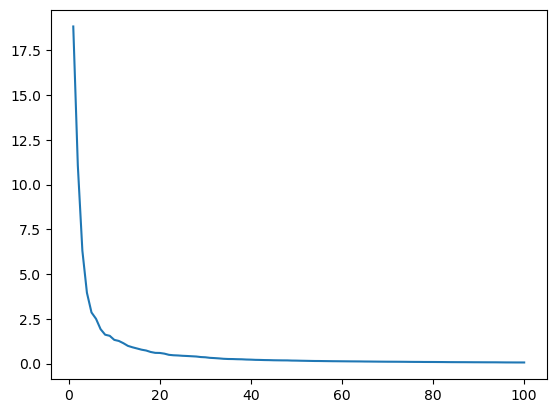
\includegraphics[width=0.75\textwidth]{eigvalues.png}
    \caption{Gráfico de scree mostrando os autovalores ordenados. O gráfico demonstra uma queda acentuada na variância explicada pelos componentes após os primeiros, seguida por um declínio mais gradual, uma forma característica de "cotovelo".} 
    \label{fig:scree}
\end{figure}

A Figura~\ref{fig:scree} mostra que os primeiros componentes principais capturam uma quantidade significativa de variância, com a variância explicada pelos componentes subsequentes diminuindo rapidamente.
Isso é típico no PCA e indica que um número muito menor de componentes pode representar uma grande parte da variabilidade dos dados. 

\section{Determinando o Número Ótimo de Componentes}
Com base na análise visual, o número ótimo de componentes foi determinado como sendo 20.
O PCA foi então reaplicado usando $n_{componentes} = 20$.

\section{Avaliação do Desempenho da Classificação}
Para avaliar a eficácia da redução de dimensionalidade, um classificador Gaussian Naive Bayes foi treinado nos dados transformados pelo PCA ($X_{pca}$ com 20 componentes). 
O desempenho foi avaliado usando validação cruzada estratificada de 10 folds (10-fold stratified cross-validation). 
A acurácia reportada da validação cruzada de 10 folds foi $0.93 \pm 0.03$.
Isso indica que o modelo alcançou uma acurácia média de 93\% com um desvio padrão de 3\% entre os folds. 

\section{Conclusão}
A aplicação do PCA reduziu significativamente a dimensionalidade do conjunto de dados Olivetti Faces de 4096 características para apenas 20 componentes principais. 
Apesar desta redução substancial, uma alta acurácia de classificação de 93\% foi alcançada usando um classificador Gaussian Naive Bayes. 
Isso demonstra que o PCA capturou com sucesso as características mais salientes dos dados, permitindo uma classificação eficiente e eficaz em uma representação de dimensionalidade muito menor. 

\end{document}